\subsection{Message Stream Controller}
\label{MessageStreamController}

The Message Stream Controller is a GUI that manipulates the message stream that it is attached to. By having other GUIs synchronize
to the same stream, this allows the user to control playback of mulitple GUIs via one interface. This is especailly useful 
when the GUIs do not expose the message stream manipulation functionality directly, like in the case of Earth Watcher. 

{\it messageStreamController} source code can be found in {\tt .\slash src\slash
clients\slash messageStreamController}. The binary produced after building is 
named {\tt messageStreamController}. This is a Qt-based application, and thus uses the Qt build system, qmake. To build: {\tt qmake, make}.

\subsubsection{Command Line Options}
\begin{itemize}
\item {\tt -h, --help}, show a usage message and exit. 
\item {\tt -s, --server}, connect to the watcher daemon at this address or hostname. Supports host:port, address:port syntax.
\end{itemize}

\subsubsection{Configuration}
\begin{itemize}
\item {\tt server}, name or ipaddress of the server to connect to.
\end{itemize}

\subsubsection{Usage}

Push the buttons, etc. 

\begin{figure}[htb]
\centering
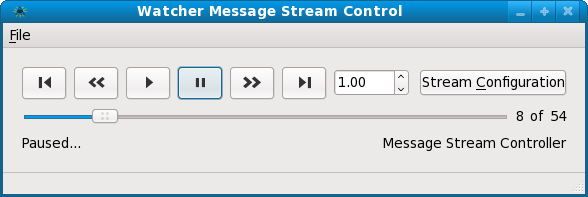
\includegraphics[width=0.8\textwidth]{messageStreamControllerMain.eps}
\caption{The main interface of messageStreamController gives playback control, playback status, and stream configuration options via a button}
\label{fig:MessageStreamControlMain}
\end{figure}

\begin{figure}[htb]
\centering
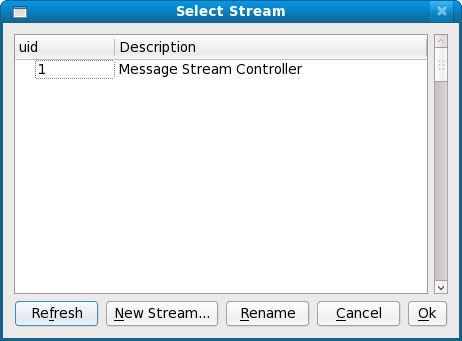
\includegraphics[width=0.5\textwidth]{messageStreamControllerStreamConfig.eps}
\caption{messageStreamController stream manipulation options include rename, new stream, choose stream from existing streams list box}
\label{fig:MessageStreamControlStreamConfig}
\end{figure}


\begin{figure}[htb]
\centering
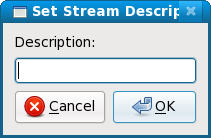
\includegraphics[]{messageStreamControllerRename.eps}
\caption{Renaming an existing stream}
\label{fig:MessageStreamControlRename}
\end{figure}

